\subsubsection{Comando LIST}

Nel messaggio di comando list non sono previsti campi aggiuntivi oltre a quello che specifica il comando.

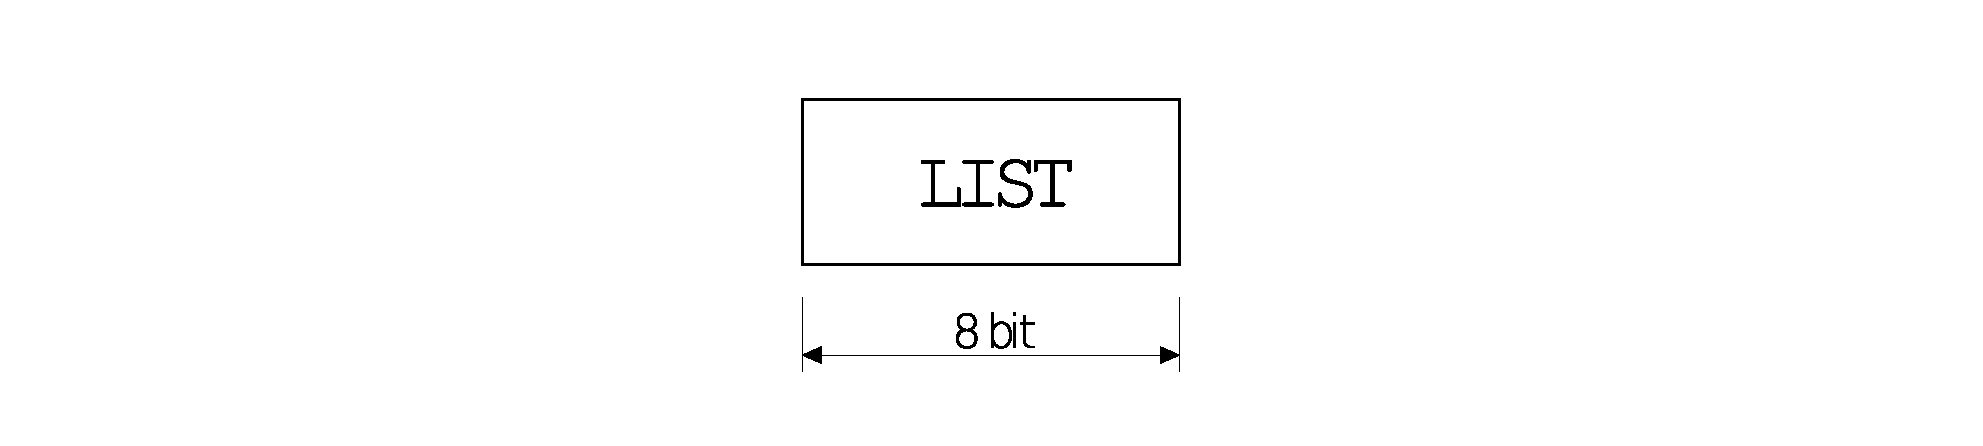
\includegraphics[scale=0.35]{images/list_client}

Il server ricevuto il comando, esegue il comando di sistema \emph{ls} redirigendo l'output sul file \emph{file\_list.txt}, dopodiché viene impostato il messaggio di risposta con la dimensione del file (campo da 64 bit) e a seguire il file contenente la lista dei file disponibili al download.

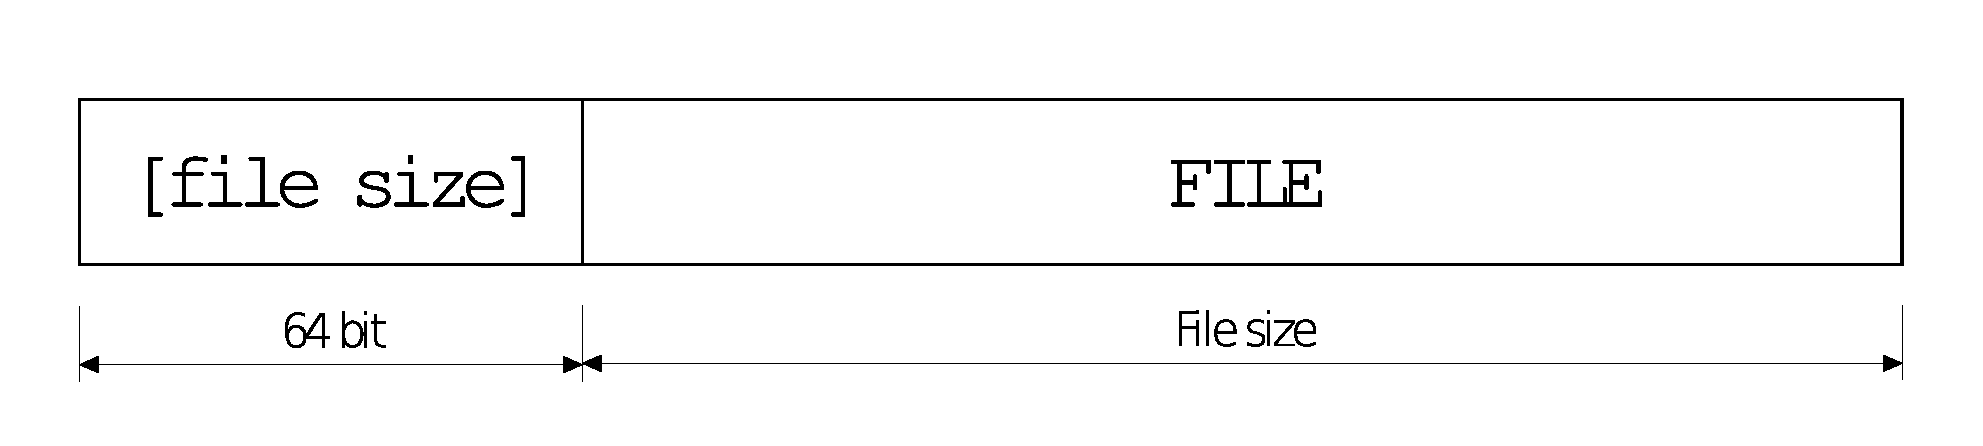
\includegraphics[scale=0.35]{images/list_server}

\begin{lstlisting}[title=clicmd.c]
void cli_list()
{
    uint8_t cmd = LIST;
    uint64_t file_size;
    char *buffer;

    /* send LIST command */
    rdt_send(&cmd, sizeof(cmd));

    /* read list size */
    rdt_recv(&file_size, sizeof(file_size));

    /* allocate buffer */
    buffer = malloc(file_size);
    if (!buffer)
        handle_error("malloc()");

    /* recv file list */
    rdt_recv(buffer, file_size);

    /* print file list and free memory */
    printf("\n%s\n", buffer);
    free(buffer);
}                                                                
\end{lstlisting}

\begin{lstlisting}[title=srvcmd.c]
void srv_list(void)
{
    int fd;
    struct stat st;
    uint64_t file_size;
    uint8_t *header;
    char *filename = "file_list.txt";

    /* execute ls command */
    char *cmd = "ls > file_list.txt";
    if (system(cmd) == -1)
        handle_error("system() - executing ls command");

    /* open the destination file of the list command */
    fd = open(filename, O_RDONLY);
    if (fd == -1)
        handle_error("open() - opening LIST file");

    /* calculate file size */
    if (fstat(fd, &st) == -1)
        handle_error("fstat() - getting LIST file stats");
    file_size = st.st_size;

    /* allocate header buffer */
    header = malloc(sizeof(file_size));
    if (!header)
        handle_error("malloc() - allocating LIST header");

    /* set the header */
    memcpy(header, &file_size, sizeof(file_size));

    /* send file and free resources */
    send_file(fd, header, file_size, sizeof(file_size));
    free(header);
    if (close(fd) == -1)
        handle_error("close() - closing file list");
}
\end{lstlisting}
